\section{The graphs, and how to read them}

All figures below are generated from the verified dynamic-world run
(\code{logs/matlab\_dynamic.csv}) by \code{make\_figures.m}.

\subsection{Reading the gaps in the data first}

Every logged series has places where it legitimately carries \emph{no}
information. Plotting those samples as if they were data produces artefacts
that look like controller behaviour but are not. Three distinct kinds:

\begin{enumerate}[leftmargin=1.9em]
\item \textbf{Sentinel gaps (value $= 99$).} A column holds 99 where the
quantity is undefined --- historically ``no mover nearby''. These are
\emph{masked} to NaN by \code{make\_figures.m} so they are simply not drawn;
unmasked, a single sentinel turns a 0--10~m axis into a 0--99 axis and
everything real becomes invisible.
\item \textbf{Semantic gaps (same column, different quantity).}
\code{dist\_to\_goal} is the \emph{max slot error} during forming (converges
to 0.3 m) and the \emph{centroid-to-goal distance} during transport (starts
at 23.9 m, converges to 0.5 m). Joined into one line, the phase boundary
shows a fake jump of $0.3 \to 23.9$~m. The figures therefore draw the two
phases as separate coloured segments with a marked boundary.
\item \textbf{Coverage gaps (metric defined only in one phase).} The
predicted mover gap was originally computed only in Phase~2 (Phase~1 logs
held a 99 placeholder), so its series started mid-run with a cliff. The
current instrument computes the same per-robot prediction during forming
too, so the metric is defined across the whole run; the value is large
(3.5~m) there because the scattered robots simply are not near movers yet.
\end{enumerate}

\begin{figure}[h]
\centering
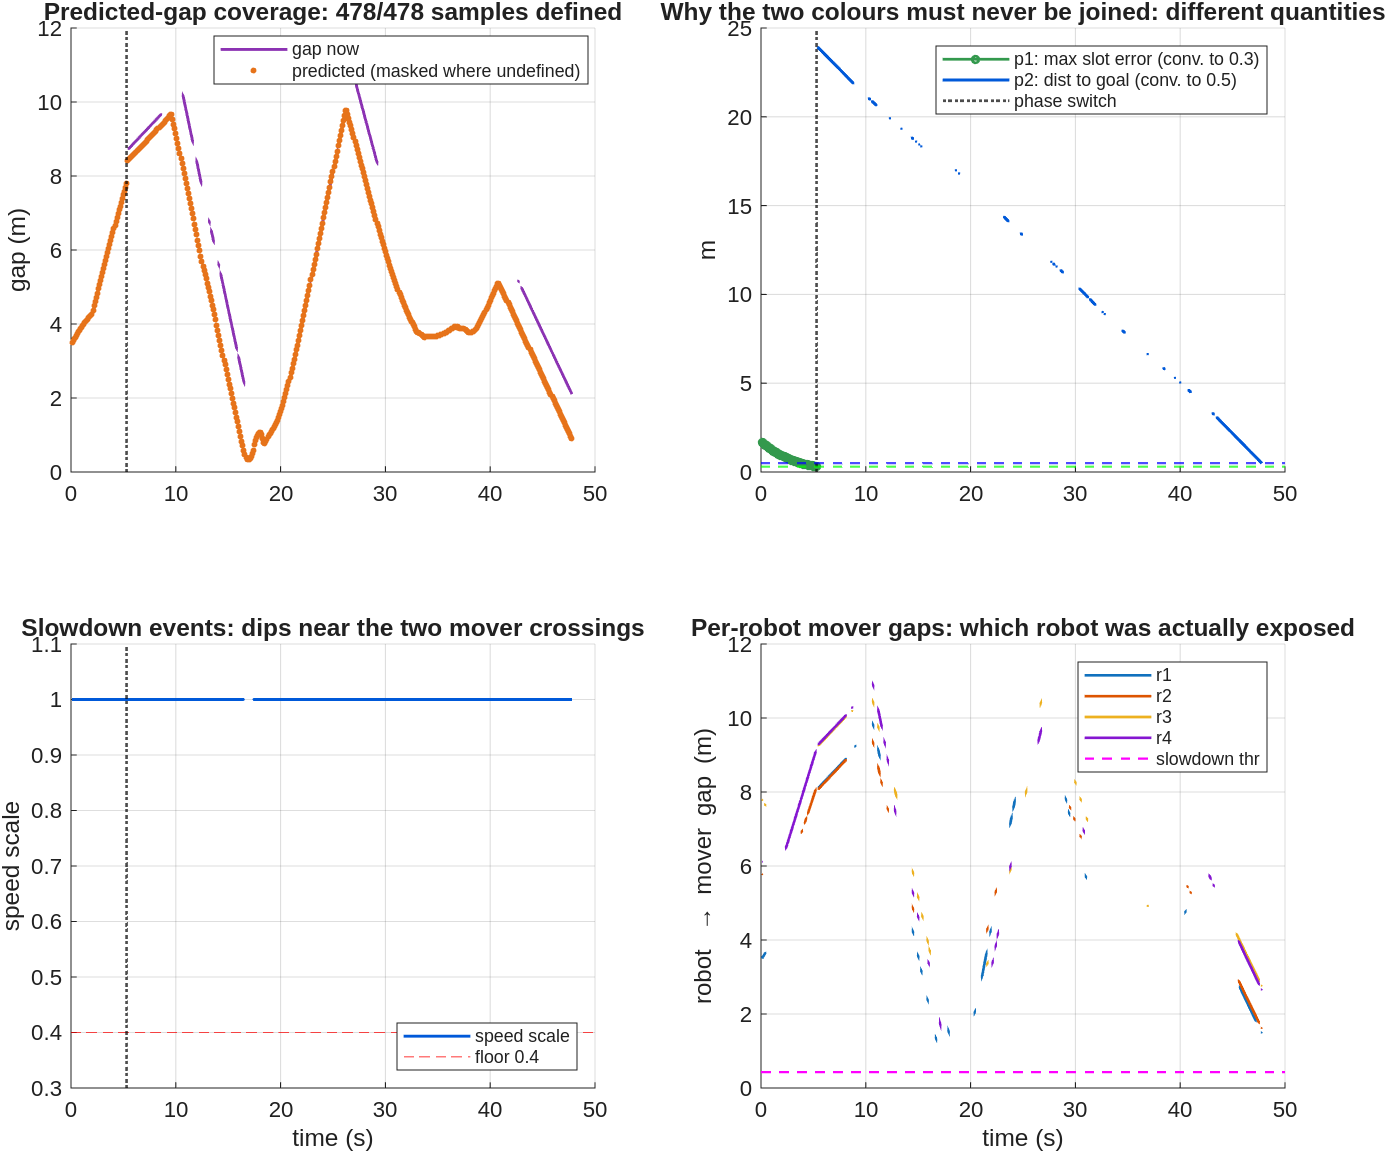
\includegraphics[width=0.94\textwidth]{figures/fig_gaps.png}
\caption{The gaps, made explicit. Top left: predicted-gap coverage against
the current gap (masked samples are simply absent). Top right: the two
semantics of the approach metric, deliberately not joined. Bottom left:
speed-scale dips at the two mover crossings. Bottom right: per-robot mover
gaps recomputed from the logged poses --- the aggregate metric hides which
robot was actually exposed.}
\label{fig:gaps}
\end{figure}

The bottom-right panel deserves a note: the logged \code{mover\_gap} is a
minimum over the whole formation. During a crossing, one robot is threatened
and the other three are fine; the aggregate says ``1.2~m'' but the per-robot
recomputation shows the exposed robot's true gap and when. Any safety argument
should be made on per-robot data.

\subsection{Trajectory map}

\begin{figure}[h]
\centering
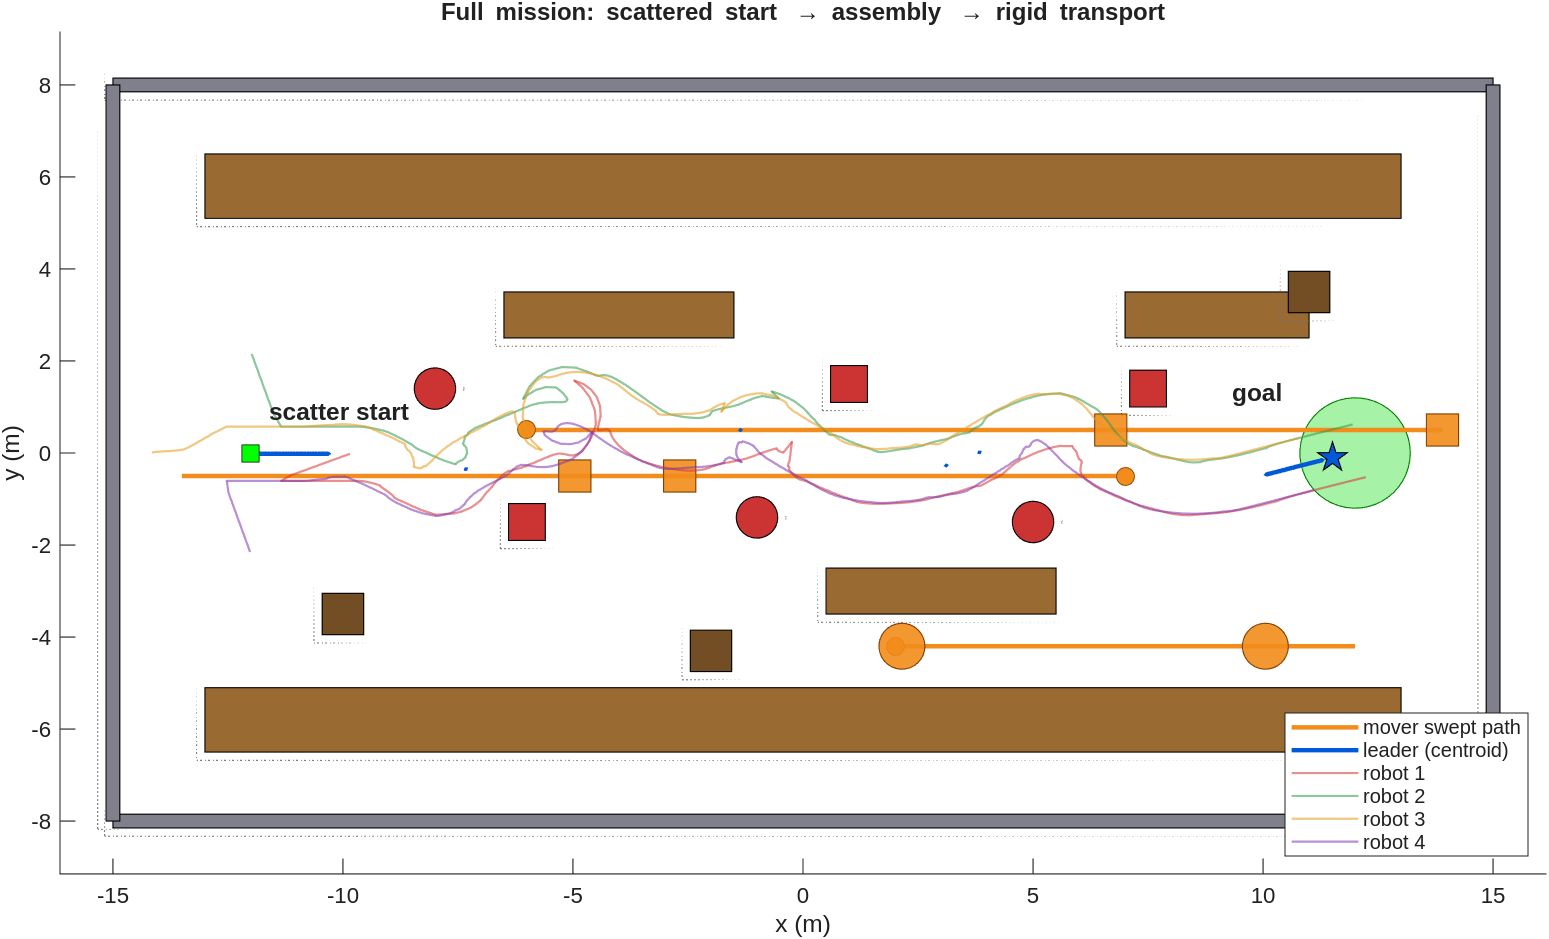
\includegraphics[width=\textwidth]{figures/fig_trajectory.png}
\caption{The whole mission. Black/dashed: warehouse. Blue line: leader
(formation-centre) trajectory. Coloured dots: the four robots during
transport. Orange: mover swept paths and poses at the two closest-approach
instants.}
\label{fig:traj}
\end{figure}

\textbf{What to look for.} (i) The coloured robot trails now cover the
\emph{whole} mission: the scatter$\to$square assembly (first $\sim$5~s of
motion, robot trails converging from the ring) and then the rigid transport.
(ii) The blue leader path bends \emph{once} around pillar4/pillar5 but is
otherwise straight: efficiency $0.93$ means avoidance was local, not global
wandering. (iii) At $x \approx -6$ and $x \approx 10.6$ the path bulges
around the orange movers --- those are the two yield events. (iv) The robot
trails stay a tight lattice through both yield events; the payload block
never clips anything.

\textbf{Failure signatures:} a leader line that doubles back (heading limit
cycle --- check the predictive scan), robot trails crossing obstacles
(collision test too weak --- is payload mode on?), or sawtooth spacing
(formation servo too stiff for the turn rate).

\subsection{Diagnostic time series}

\begin{figure}[h]
\centering
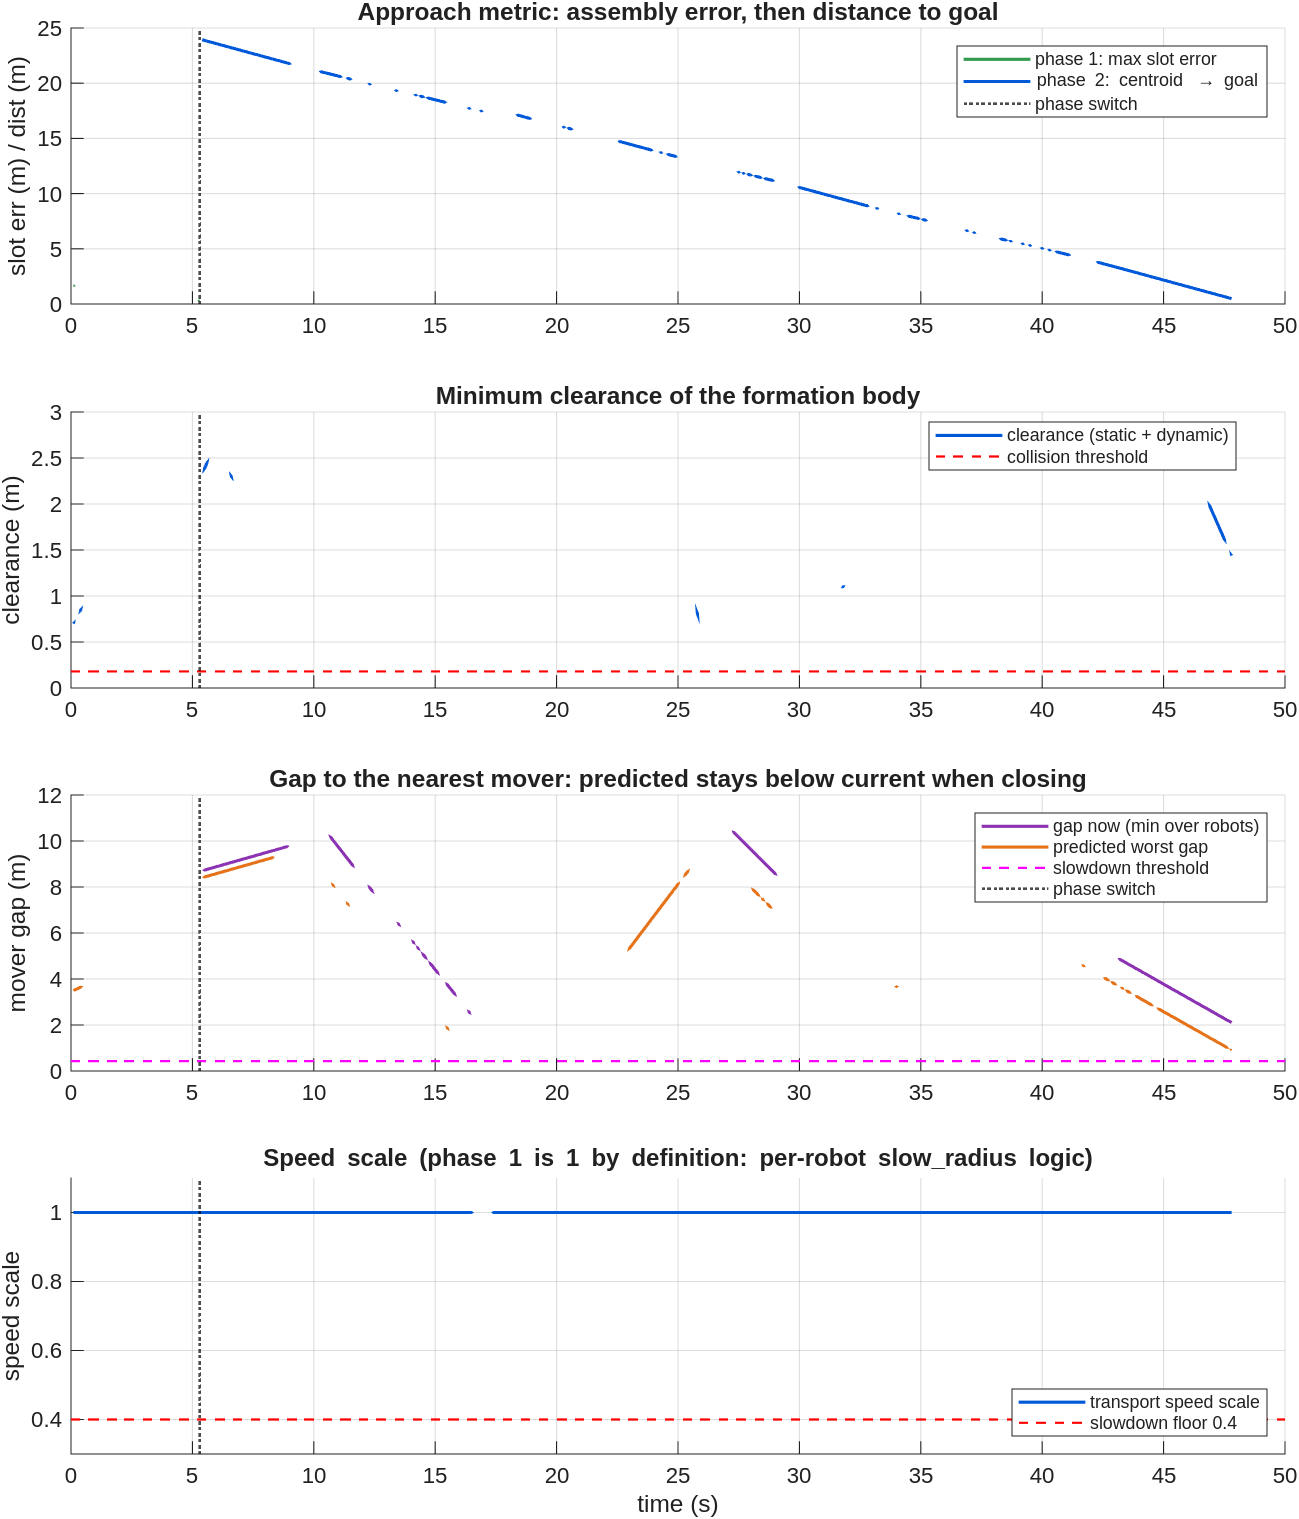
\includegraphics[width=0.86\textwidth]{figures/fig_diagnostics.png}
\caption{Top to bottom: the approach metric (green = slot error in forming,
blue = distance to goal in transport, boundary marked), formation clearance
across the whole run, mover gap now vs predicted, and the transport speed
scale. Vertical dotted lines mark the phase switch at $t = 5.4$~s.}
\label{fig:diag}
\end{figure}

\begin{itemize}[leftmargin=1.6em]
\item \textbf{Approach metric (top).} Two different quantities, two
colours, never joined. The green segment converges to the 0.3 m formation
tolerance; the blue segment then runs 23.9 m $\to$ 0.49 m. Flats in the blue
segment while clearance stays healthy mean a stall (escape logic engaged); a
rise means avoidance was worth the detour --- match it against the clearance
panel directly below.
\item \textbf{Clearance (second).} The red dashed line is the collision
threshold (robot radius). The curve dipping \emph{toward} it at the chicane
and at the mover crossings is correct --- the corridor physically pinches to
2.45 m, and the block needs 2.02 m of it. Minimum 0.51 m means the
controller used 72\% of the available margin at the worst instant and never
crossed the line.
\item \textbf{Mover gaps (third).} Purple: current gap (min over robots).
Orange: predicted worst gap over the 1 s lookahead --- it sits \emph{below}
the purple line exactly while a mover is closing, which is the whole point
of prediction. The magenta dashed line is the slowdown threshold. The two
dips are the two movers; the predicted minimum of 0.33 m is what triggered
the slowdown, while the gap that actually materialised never went below
1.22 m.
\item \textbf{Speed scale (bottom).} 1.0 everywhere except the dips near the
mover crossings (minimum 0.61). Phase 1 is constant 1 by definition ---
forming speed is governed by each robot's own slow-radius logic, not the
transport slowdown. The 0.4 floor is never reached in this run: the yield
was resolved by steering, with slowdown as assist rather than as the primary
mechanism.
\end{itemize}

\subsection{Per-robot and inter-robot graphs}

\begin{figure}[h]
\centering
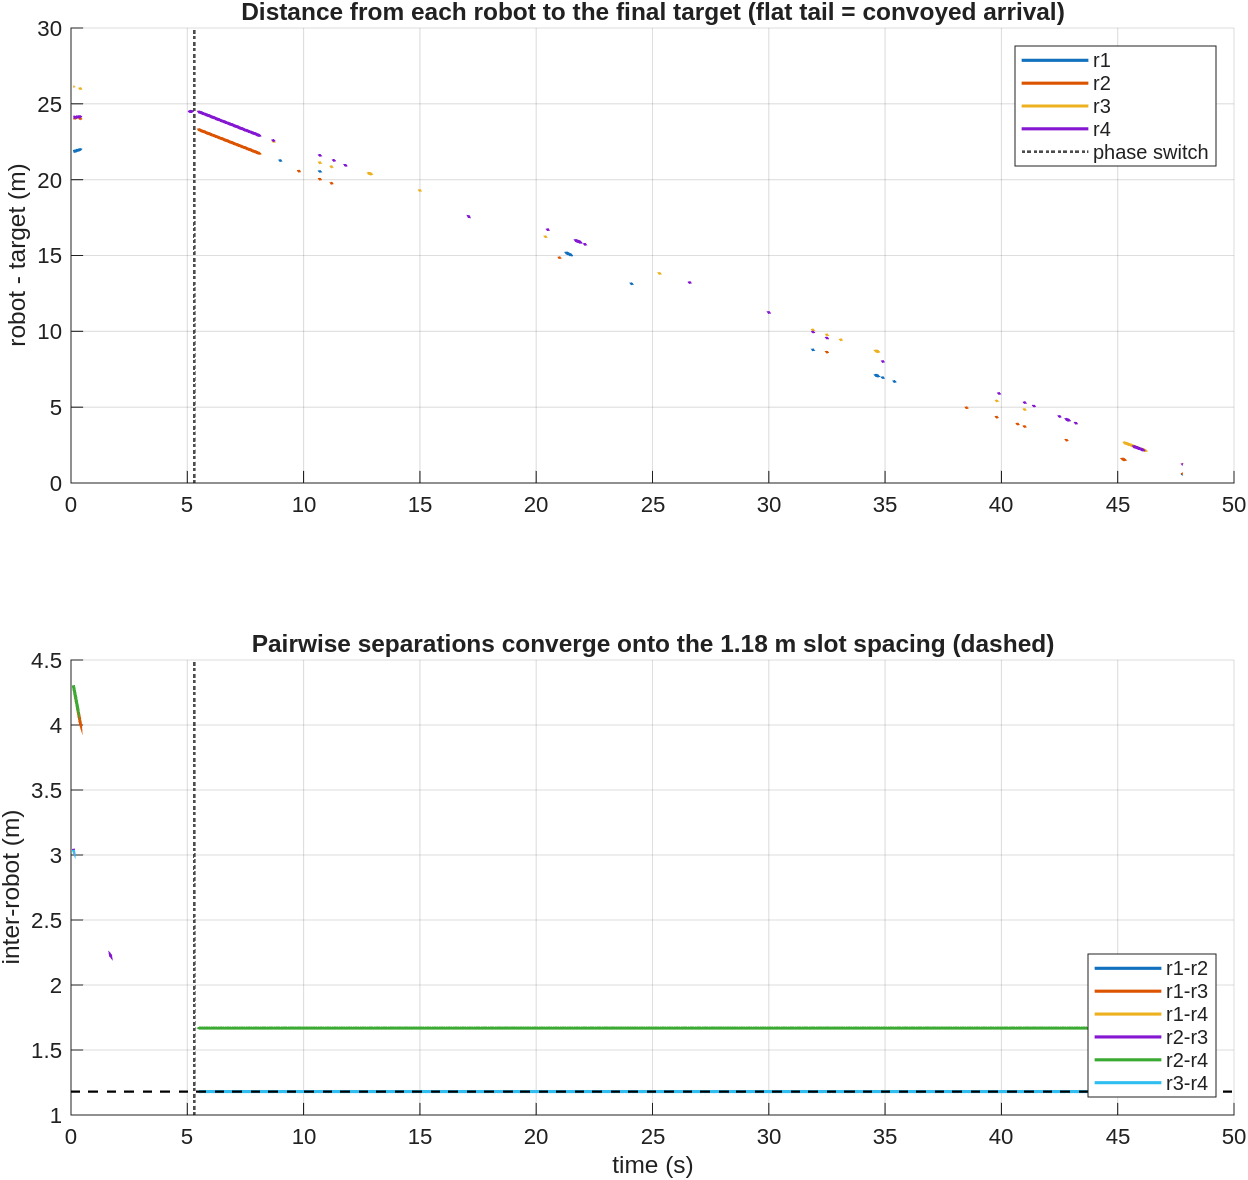
\includegraphics[width=0.86\textwidth]{figures/fig_graphs.png}
\caption{Top: distance from each robot to the final target. Bottom: pairwise
robot separations against the nominal slot spacing (dashed).}
\label{fig:graphs}
\end{figure}

\textbf{Top panel.} Four curves, one per robot. They start at different
ranges (scattered start), converge to nearly identical values within the
first seconds (assembly), then decrease together --- the signature of a rigid
body translating. The flat tail at $\approx 0.5$~m is the goal-reaching
offset: the leader stops when the \emph{centroid} is within $0.5$~m, so each
robot sits at its slot radius from the goal. Curves that cross during
transport mean the assignment permuted mid-run (should not happen; slots are
fixed after Phase~1).

\textbf{Bottom panel.} Six curves, one per robot pair. In the kinematic model
these are constant by construction --- they oscillate mildly only during
assembly and at yield events where the frame heading swings. The dashed line
is the nominal spacing $1.18$~m; all six curves sit on it after
$t \approx 5$~s. In a ROS~2 replication this panel is \emph{the} formation
quality metric: \code{formation\_rms} in \code{compare\_runs.m} is exactly
the RMS deviation of these six curves from their own mean, and any structural
difference between the stacks shows here first.

\subsection{Formation geometry}

\begin{figure}[h]
\centering
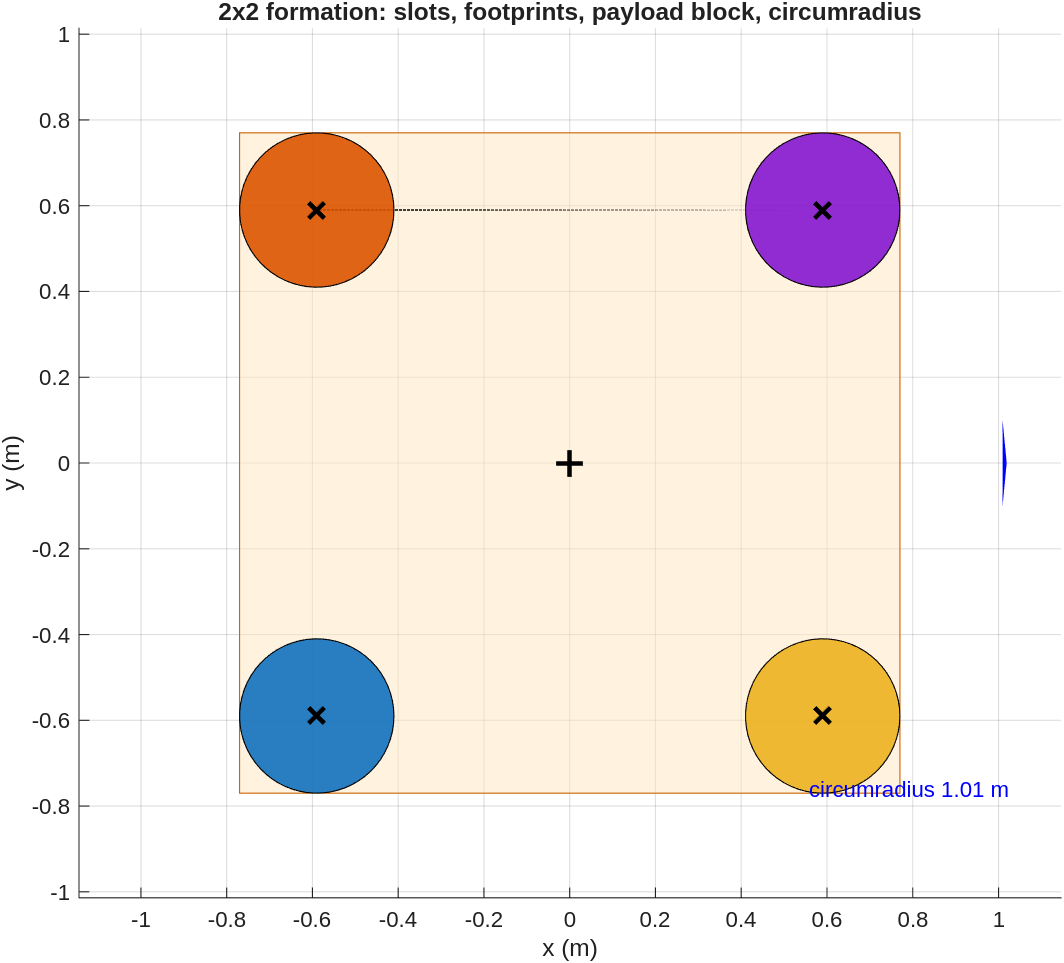
\includegraphics[width=0.62\textwidth]{figures/fig_formation.png}
\caption{The transported body. Filled circles: robot footprints at true size.
Orange: the payload block (slot square inflated by the robot radius). Blue:
the effective circumradius used for VFH enlargement and feasibility.}
\label{fig:form}
\end{figure}

This figure explains \emph{why} the spacing is what it is. The quantity that
must fit through a corridor is the circumradius
$c = 0.59\sqrt{2} + 0.18 = 1.01$~m --- not the half-width --- because the
block rotates. The bottleneck is $1.22$~m, so the margin is $0.21$~m: any
controller that drifts more than that in a turn physically cannot pass, which
is why the feasibility check runs before the simulation and why the spacing
auto-fixes to $1.18$~m rather than a round number.

\subsection{p-VFH histogram and the predictive scan}

\begin{figure}[h]
\centering
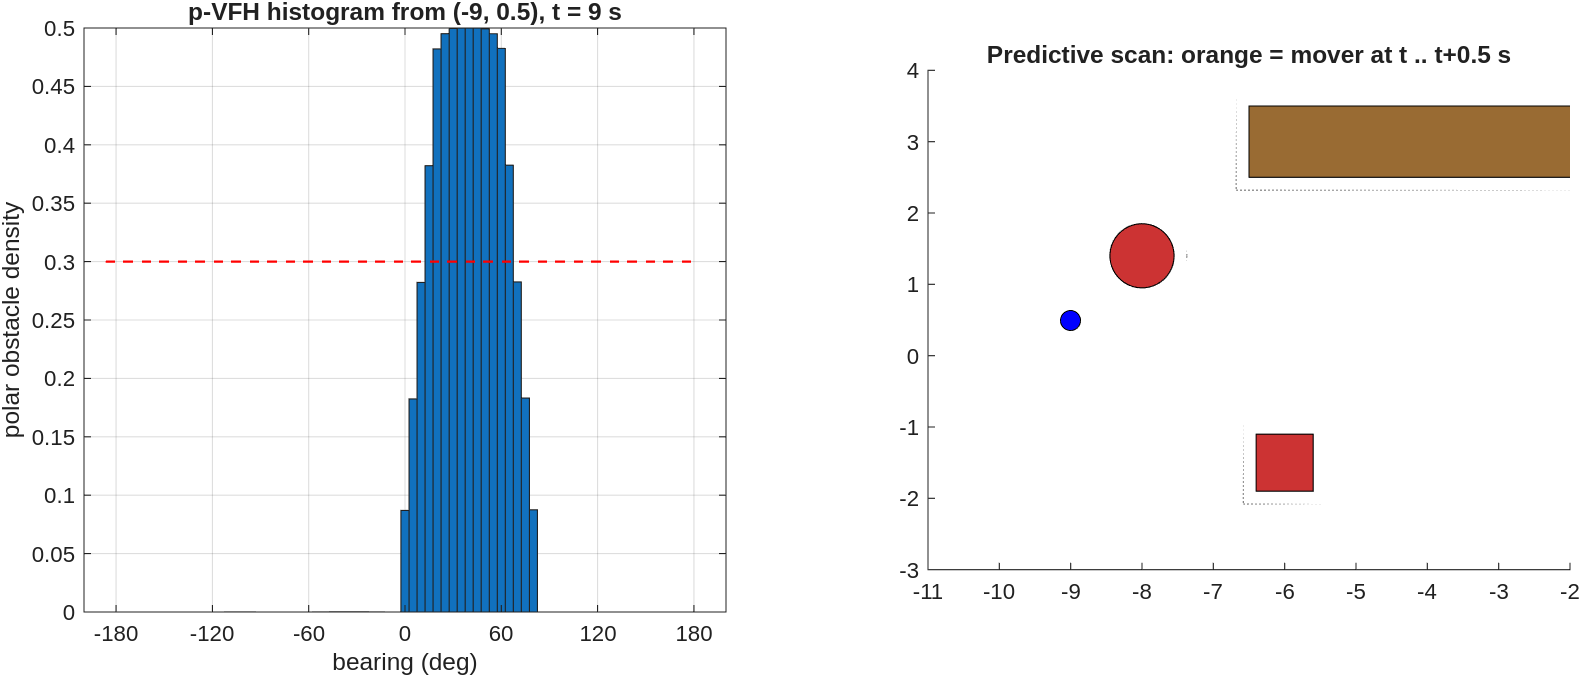
\includegraphics[width=\textwidth]{figures/fig_vfh.png}
\caption{Left: the polar obstacle density at $t = 9$~s from the formation
start position. Right: the scene --- orange rings are the mover at
$t \dots t + 0.5$~s.}
\label{fig:vfh}
\end{figure}

\textbf{Left panel.} Height is danger: sectors above the red dashed line
($\tau = 0.3$) are blocked, sectors below are candidate valleys. The broad
wall of density around $0^\circ$ is the approaching mover plus pillar1; the
walls at $\pm 90^\circ$ are the shelf faces. The controller picks the valley
closest to the goal bearing (toward $0^\circ$ here) --- so the histogram must
show a \emph{gap} between the mover and the shelves for the formation to
slip through; if the mover is centred in the aisle, no gap exists and the
yield (slowdown + detour) happens instead.

\textbf{Right panel.} The orange rings are the mover at six instants over the
prediction horizon. The nearest ring is where an instantaneous scan would see
it; the rings marching toward the robot are what \code{pvfh\_predict}
actually feeds into the histogram --- the beam keeps the \emph{nearest
blocking instance over the horizon}, which is how the controller reacts to
where the obstacle \emph{will be}.
